%--------------------
% Packages
% -------------------
\documentclass[7pt,a4paper]{article}
\usepackage[utf8x]{inputenc}
\usepackage[T1]{fontenc}
%\usepackage{gentium}
\usepackage{mathptmx} % Use Times Font


\usepackage[pdftex]{graphicx} % Required for including pictures
\usepackage[swedish]{babel} % Swedish translations
\usepackage[pdftex,linkcolor=black,pdfborder={0 0 0}]{hyperref} % Format links for pdf
\usepackage{calc} % To reset the counter in the document after title page
\usepackage{enumitem} % Includes lists
\usepackage{amssymb}
\usepackage{amsfonts}
\usepackage{subcaption} 
\usepackage{float}  


\frenchspacing % No double spacing between sentences
\linespread{1} % Set linespace
\usepackage[a4paper, lmargin=0.1666\paperwidth, rmargin=0.1666\paperwidth, tmargin=0.1111\paperheight, bmargin=0.1111\paperheight]{geometry} %margins
%\usepackage{parskip}

\usepackage[all]{nowidow} % Tries to remove widows
\usepackage[protrusion=true,expansion=true]{microtype} % Improves typography, load after fontpackage is selected

\usepackage{lipsum} % Used for inserting dummy 'Lorem ipsum' text into the template


%-----------------------
% Set pdf information and add title, fill in the fields
%-----------------------
\hypersetup{ 	
pdfsubject = {Medical Robotics},
pdftitle = {Closed-Loop BCI-Triggered System with Soft-Robotic Glove for after-stroke rehabilitation},
pdfauthor = {Flavio Massaroni}
}

%-----------------------
% Begin document
%-----------------------
\begin{document}

\title{Closed-Loop BCI-Triggered System with Soft-Robotic Glove for after-stroke rehabilitation}
\author{Flavio Massaroni}
\date{}

\maketitle

\section{Clinical Need}
Stroke represents a major cause of long-term neurological disability globally. 
As evidenced by epidemiological data from the World Stroke Organization [1], the socio-health impact of
this pathology is constantly growing: over 93 million cases prevalent, some 160 million years of life lost to disability
(DALYs) and a cost estimated global economic of more than US\$ 890 billion. 

Between 55\% and 75\% ofsurvivors have chronic upper limb motor deficit which compromises autonomy 
in daily activities (ADL) [12]. Donkor [2] contextualize this figure in the perspective of quality of life:
stroke is the second cause of death at the world and causes severe permanent disability in about half 
of the survivors, with high impact on autonomy, working life and the care burden on family members.

This combination of high prevalence and high residual disability justifies 
the search for advanced technological solutions that can deliver portable therapy with 
an intensity comparable to that of departments of specialized rehabilitation.
Recent clinical research indicates that the effectiveness of traditional rehabilitation treatments is severely 
limited by a therapeutic dosage deficit. 
The systematic analysis conducted by Newton et al. [3]
highlights how the actual time spent on active therapeutic exercise (time on task) within conventional
sessions varies on average between 8 and 44 minutes per day — significantly lower than recommended doses to 
induce cortical reorganization stable. A clinical paradox emerges: patients with more severe impairment receive 
doses of significantly lower active therapy precisely because of the high effort required without tools modular 
assistance.


\section{Current Standard of Care and Its Limitations}

The current standard of post-stroke upper limb rehabilitation combines 
conventional physiotherapy with commercially available robotic orthoses. 
Both approaches share a critical failure mode: they address the peripheral 
component of motor recovery while neglecting its central requirement.

Newton et al.~\cite{newton2023dose} quantify this dose gap: effective 
active therapy time in conventional care averages 8--44 minutes per day — 
far below the repetition volume required to induce stable cortical 
reorganization. After discharge, most patients receive virtually no 
structured rehabilitation.

The robotic hardware available today does not close this gap. Wang et 
al.~\cite{wang2023effectiveness} compared a passive soft-robotic glove 
against repetitive transcranial magnetic stimulation (rTMS) in patients 
with severe upper limb dysfunction. The passive glove improved 
Fugl-Meyer Assessment scores (FMA-UE) by facilitating joint mobilization, 
but produced no significant changes in Resting Motor Threshold (RMT) or 
Motor Evoked Potential (MEP) amplitude — the markers of cortical synaptic 
excitability. The glove moves the hand, it does not engage the brain.

The neurobiological explanation is well established. Long-term motor 
recovery depends on Hebbian plasticity (Spike-Timing-Dependent Plasticity, 
STDP): stable synaptic modifications require temporal coincidence — within 
approximately 300\,ms — between the pre-synaptic signal (motor cortex 
activation associated with movement intention) and the post-synaptic 
afferent feedback generated by the actual limb movement 
\cite{biasiucci2018brain, krueger2024hebbian}. In the $\mu$ (8--12\,Hz) 
and $\beta$ (13--30\,Hz) bands, Motor Imagery manifests as event-related 
desynchronization (ERD) over contralateral motor areas (C3/C4). When a 
BCI detects this ERD and uses it as an instantaneous trigger, the Hebbian 
coincidence window is realized. A random or sham activation produces no 
significant increase in $\beta$-band corticomuscular coherence 
\cite{krueger2024hebbian} and no relevant clinical improvement 
\cite{kim2025efficacy}.

The biomarker of this reorganization is measurable in real time: Rustamov 
et al.~\cite{rustamov2025ipsihand} demonstrate that theta-gamma 
cross-frequency coupling (CFC) over C3/C4 increases proportionally to 
motor recovery across BCI sessions, confirming CFC as a neurobiological 
proxy for treatment efficacy. The mechanism exists, is validated, and is 
quantifiable. The gap is not biological — it is a delivery problem.

% ---------------------------------------------------------------
\section{The Human Limitation Being Addressed}
% ---------------------------------------------------------------

The mechanism described above requires three conditions that no human 
operator can reliably provide in an unsupervised home setting:

\textbf{(1) Continuous presence.} The Hebbian contingency must be enforced 
at every repetition across sessions of 30--45 minutes, 3--5 times per week, 
for months. A trained therapist cannot be physically present at the 
patient's home at this frequency — this is precisely the dose gap 
documented by Newton et al.~\cite{newton2023dose}.

\textbf{(2) Sub-300\,ms reactive latency.} The BCI trigger must fire 
within the Hebbian coincidence window \cite{krueger2024hebbian}. To allow 
a consistent satisfaction of this condition, a robotic solution is the 
most reliable means of automatic response.

\textbf{(3) Operator-independent consistency.} Outcome variability in 
conventional rehabilitation is partially attributable to inter-therapist 
inconsistency in task delivery and feedback timing \cite{newton2023dose}. 
A closed-loop BCI system applies identical contingency criteria at every 
trial, eliminating this source of variance. Ren et al.~\cite{ren2024effect} 
confirm in a meta-analysis of 10 RCTs (290 patients) that BCI-triggered 
intervention outperforms conventional therapy (SMD\,=\,0.50, 95\,\% CI: 
0.26--0.73), with effect size directly linked to contingency fidelity.

The robot is not a substitute for clinical judgment — the therapist remains 
in the loop asynchronously via remote dashboard. It is a substitute for 
physical presence and consistanc and automatic reactivity.


% ---------------------------------------------------------------
\section{Proposed Robotic Solution}
% ---------------------------------------------------------------

To overcome the issue, the proposed solution is a BCI-Triggered system with a Soft Robotic Glove. This is the direct consequence
of the need to satisfy the time gap consistency and the continuative dose during years.
The device is classified as a wearable, domiciliary and supervised. It is used in autonomous session of 30-45 minutes per 3-5 times per week, 
without the clinitian presence. An GUI is used to set up and start up the session, and the clinitian monitors during time with a
claude communication.

\subsection{Kinematic Architecture}

The architecture is a soft-robotic pneumatic wearable glove, modelled as a sytem of serial kinematic chain anchored 
to a fixed palm \cite{proietti2024combining, fiska2025integration}.
The choice of using a pneumatic network (PneuNet) is dictated by the need of intrinsic security and passive adaptability to variable geometries in 
an unsupervised environment.

The geometric model replicates human anatomy with 3 Degrees of Freedom (DoFs) for each of the 4 fingers (MCP, PIP, and DIP joints) 
and 2 DoFs for the thumb (CMC and MCP joints), reaching a total of 14 kinematic DoFs. However, the system is intentionally under-actuated, 
employing a single independent pneumatic channel per digit to yield 5 active DoFs. The complexity-benefit trade-off of this design is governed 
by three primary factors:

\begin{enumerate}
    \item \textbf{Biological Synergies:} Neurophysiological studies (e.g., Santello et al. \cite{santello1998postural}) demonstrate that the 
    central nervous system controls hand grasping through low-dimensional synergistic patterns rather than isolated joint control. 
    Actuating 14 joints independently is redundant for post-stroke rehabilitation, which focuses on restoring gross functional synergies
    for Activities of Daily Living (ADLs).
    \item \textbf{Embodied Intelligence:} The PneuNet architecture exploits morphological computation. Upon pressurization, 
    fluid redistribution within the elastomeric chambers naturally conforms to the object's geometry, 
    bypassing the need for high-density sensor arrays or complex multi-joint control algorithms.
    \item \textbf{Usability and Weight Constraints:} Implementing 14 active lines would introduce excessive hardware overhead.
    Minimizing weight is crucial to prevent muscular fatigue and abnormal compensatory movements at the shoulder, ensuring autonomous, 
    single-handed donning by hemiparetic patients at home.
\end{enumerate}

\begin{figure}[H]
     \centering
     \captionsetup{aboveskip=2pt, belowskip=2pt} % Compatta le didascalie
     \begin{subfigure}[t]{0.45\textwidth}
         \centering
         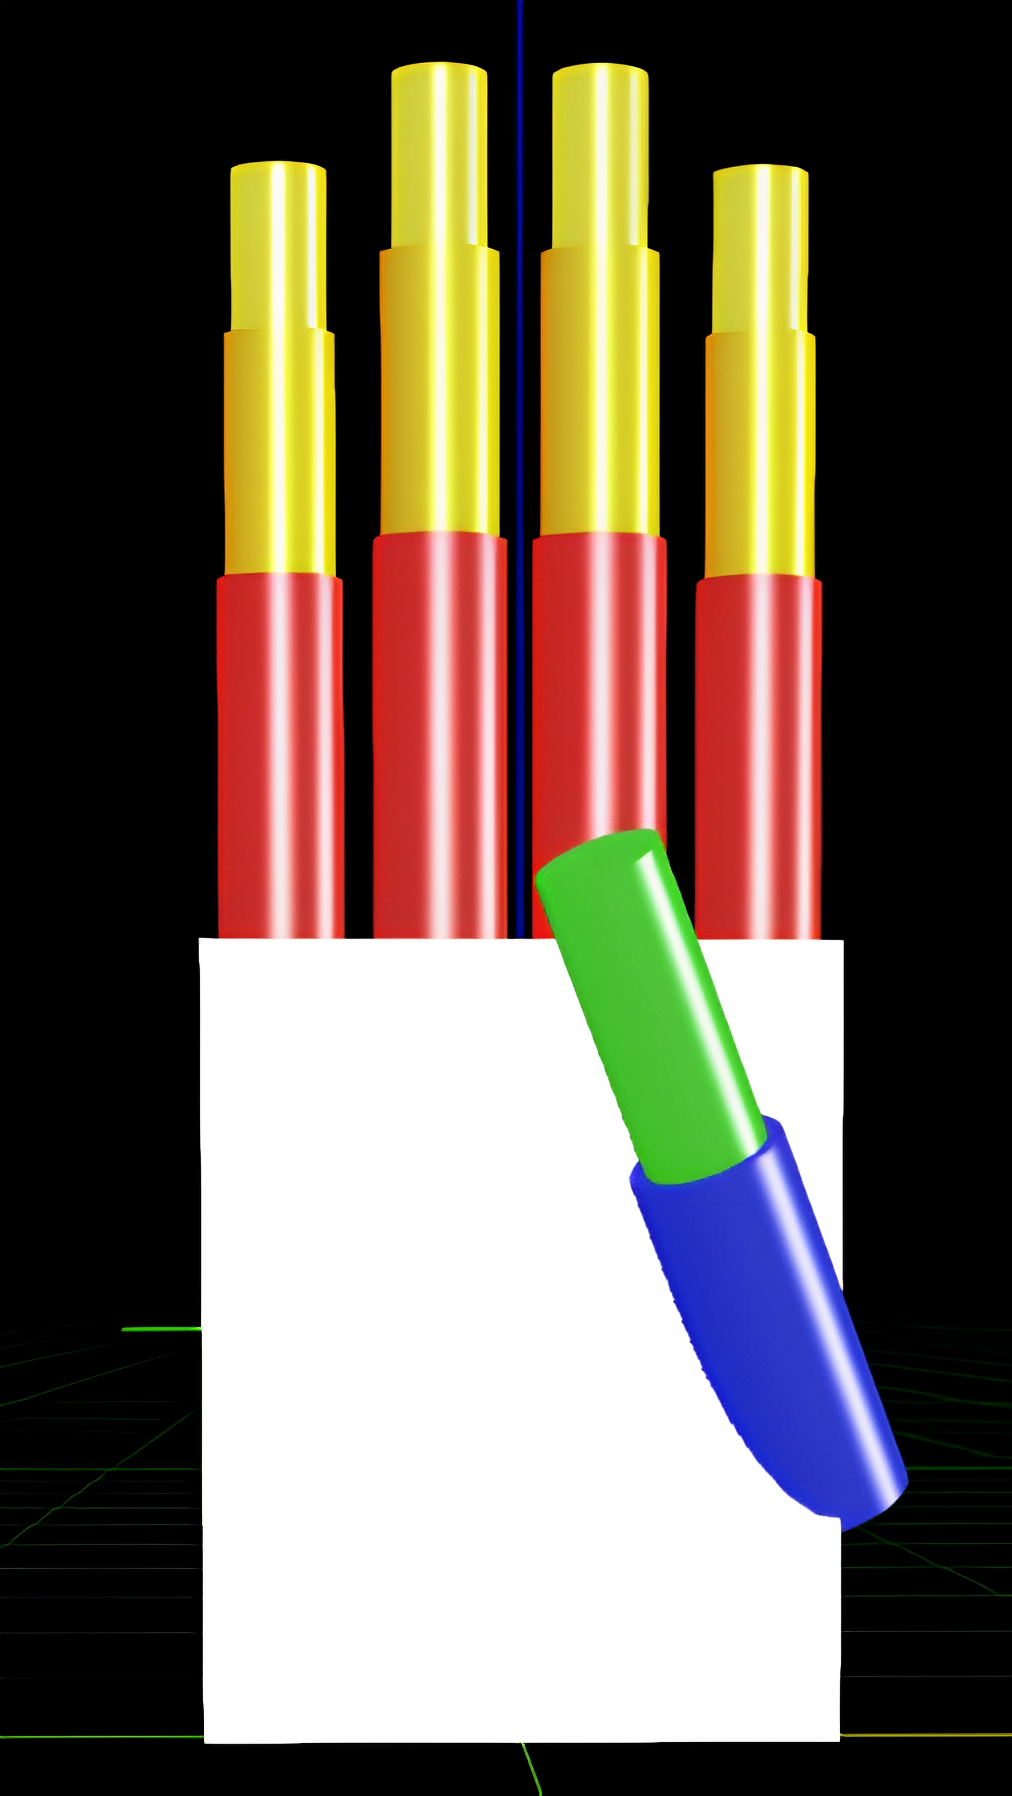
\includegraphics[width=0.9\textwidth, trim=0 30 0 30, clip]{hand_view1.png}
         \caption{Frontal view}
     \end{subfigure}
     \hfill
     \begin{subfigure}[t]{0.45\textwidth}
         \centering
         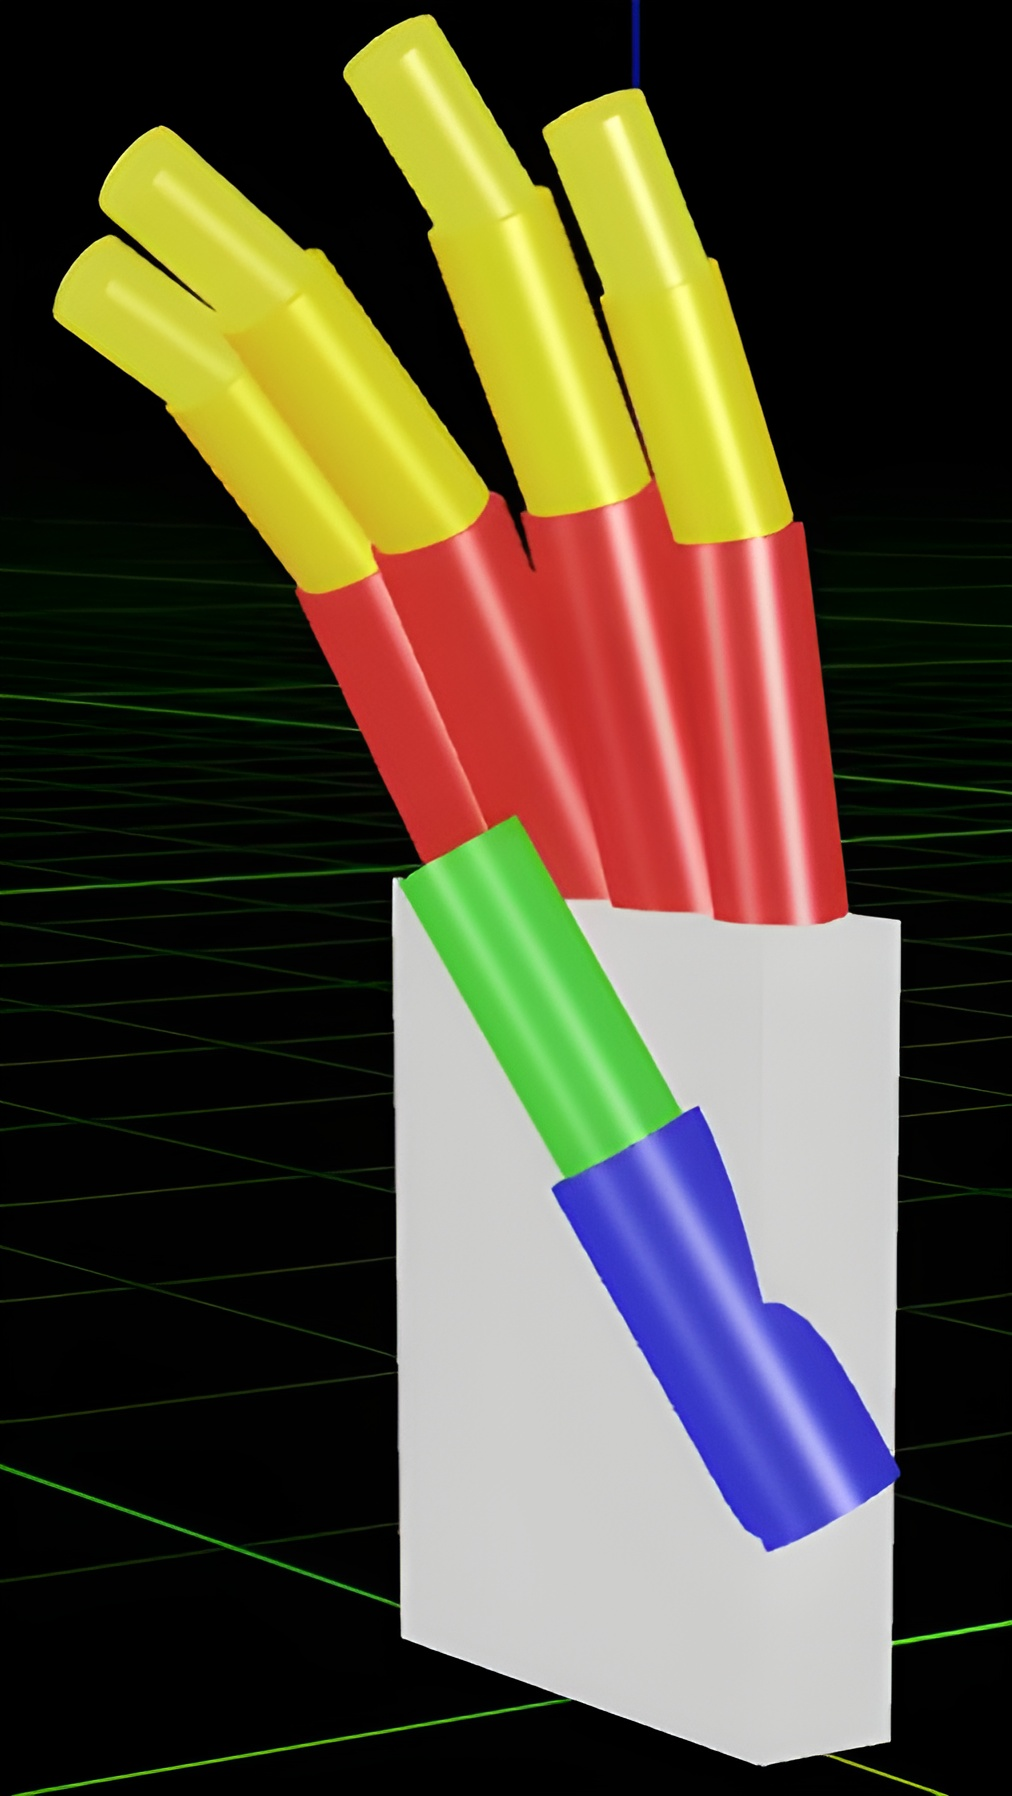
\includegraphics[width=0.9\textwidth, trim=0 30 0 30, clip]{hand_view2.png}
         \caption{Lateral view, showing joint flexion}
     \end{subfigure}
     \caption{URDF kinematic model of the robotic glove.}
     \label{fig:urdf_model}
     \vspace{-5pt}
\end{figure}

Mathematically, this under-actuation defines a constrained kinematic mapping where the joint space $q \in \mathbb{R}^{14}$ is
coupled to the actuator pressure space $u \in \mathbb{R}^{5}$ via a non-linear vector function:
\begin{equation}
q = g(u)
\end{equation}
where the passive elasticity of the silicone elastomer acts as a virtual restoring spring,guaranteeing a unique, statically stable equilibrium
configuration for each input pressure vector $u$.

\subsection{Sensing and Biomechanical Safety}

System sensing is categorized into two levels: neurological sensing (EEG) and local biomechanical sensing. To ensure patient safety in the absence of a clinician, the firmware implements three quantitative mechanisms in compliance with active medical device standards (IEC 60601-1) and IEC 62304 software guidelines. The system is designed to achieve the Performance Level required by ISO 13849:

\begin{itemize}
    \item \textbf{Admittance Control ($F \rightarrow v$):} Integrated palmar piezoelectric sensors measure interaction forces, dynamically modulating pneumatic pressure to ensure glove compliance; the system automatically yields to spastic resistance, prioritizing patient safety and joint protection. Kinematic joint boundaries defined in the URDF model serve as software-enforced virtual fixtures.
    \item \textbf{Fail-Safe EEG:} The system continuously monitors electrode impedance and signal quality (SNR). In the event of signal loss (1\,s timeout), all pneumatic valves are exhausted within 200\,ms, ensuring the device cannot execute non-intentional autonomous movements.
    \item \textbf{Emergency Stop:} A physical, high-visibility emergency button is located on the device controller. Accessible with the patient's unaffected hand, it immediately cuts power to the valves and exhausts residual pneumatic pressure, independently of the software state.
\end{itemize}

While EEG-based BCI for post-stroke rehabilitation is a safe and clinically established modality, 
the primary challenge lies in achieving robust decoding rather than biological feasibility. 
Cortical lesions often trigger neuroplastic reorganization, which can alter the amplitude and spatial topography of Motor Imagery signals. 
To address this inter-patient variability, our system employs an adaptive Linear Discriminant Analysis (LDA) classifier. 
This model dynamically calibrates to the patient’s specific, reorganized neural patterns, effectively compensating for post-lesional 
cortical shifts and ensuring high decoding accuracy despite the altered brain activity.


\subsection{Level of Autonomy, EEG Interface, and Inclusion Criteria}

The system operates at \textbf{Level of Autonomy 2 (Shared Control)} according to the Troccaz classification: 
the patient retains high-level decisional control by generating motor intent, while the robot autonomously manages low-level execution 
(pressure trajectories, force sensor monitoring, and feedback timing).

The system cannot operate at LoA 3 or higher because autonomous actuation, decoupled from cortical intent, 
would violate the Hebbian plasticity principle. A robotic glove moving without the patient's active intent would provide 
passive rehabilitation rather than neuroplastic training \cite{biasiucci2018brain, krueger2024hebbian}.
 Thus, LoA 2 is not a design compromise; it is the autonomy level required to induce neuroplasticity.

To ensure autonomous self-donning, the system utilizes a pre-shaped rigid-shell EEG headset with spring-loaded 
dry electrodes. The mechanical structure guides the headset into the correct position on the C3/C4 
sites within 2 minutes, removing the need for conductive gel or high-precision alignment.

\paragraph{Inclusion Criteria as Design Specification}

Autonomous donning assumes sufficient function in the contralateral hand, 
which is implicit in the primary clinical inclusion criterion (patients must be capable of single-handed operation). 
The system is therefore indicated for patients with \textbf{unilateral hemiparesis}. Patients with severe bilateral paralysis are
excluded by the device's inherent design, not by a technological limitation. This clinical boundary is an intentional design specification.

Remote clinical supervision is conducted via an \textbf{asynchronous cloud-based dashboard},
allowing clinicians to regulate virtual fixtures (angular limits, admittance thresholds), review session logs, 
and personalize task parameters \cite{proietti2024combining}. Patient progress is visualized through simplified traffic-light 
feedback cues displayed on a tablet.


\begin{figure}[ht]
    \centering
    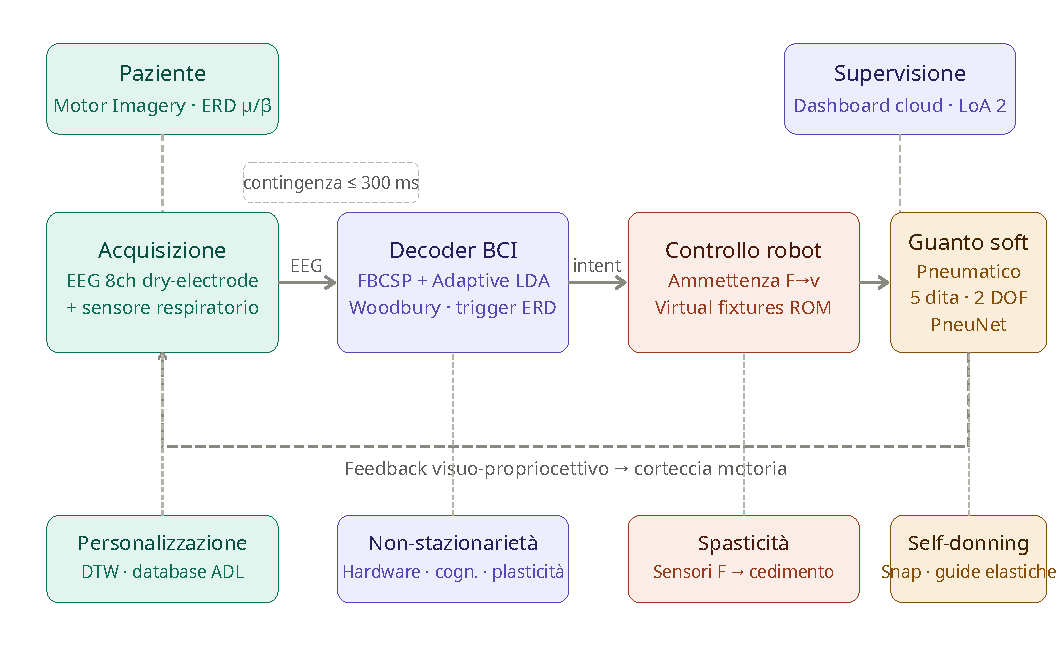
\includegraphics[width=\textwidth]{bci_glove_system_diagram_v2.pdf}
    \caption{Closed-loop architecture of the BCI-SRG system. Key components: (1) respiratory-synchronized EEG acquisition, (2) FBCSP-based adaptive LDA decoder, (3) safety controller integrating virtual fixtures and admittance control, and (4) the pneumatic soft glove. Dashed lines illustrate the visuo-proprioceptive feedback loop. Target end-to-end latency is $\leq 300$\,ms to satisfy Hebbian contingency requirements \cite{biasiucci2018brain}.}
    \label{fig:architettura}
\end{figure}


\newpage
\bibliographystyle{unsrt}

\begin{thebibliography}{1}
\small
\setlength{\itemsep}{0pt}
\setlength{\parsep}{0pt}
\setlength{\parskip}{0pt}
\setlength{\leftmargin}{0pt}
\addtolength{\leftmargin}{\labelwidth}
\addtolength{\leftmargin}{\labelsep}
\renewcommand{\refname}{Bibliografia}

\bibitem{feigin2025world}
Valery~L. Feigin et al.
\newblock World stroke organization: Global stroke fact sheet 2025.
\newblock {\em Int. J. Stroke}, 20(2):132--144, 2025.

\bibitem{donkor2018stroke}
Emmanuel~S. Donkor.
\newblock Stroke in the 21st century: burden, epidemiology, and quality of life.
\newblock {\em Stroke Res. Treat.}, 2018:3238165, 2018.

\bibitem{newton2023dose}
Sarah~P. Newton et al.
\newblock Dose, content, and context of usual care in stroke upper limb motor interventions: A systematic review.
\newblock {\em Clin. Rehabil.}, 37(11):1437--1450, 2023.

\bibitem{biasiucci2018brain}
A.~Biasiucci et al.
\newblock Brain-actuated functional electrical stimulation elicits lasting arm motor recovery after stroke.
\newblock {\em Nat. Commun.}, 9:2421, 2018.

\bibitem{krueger2024hebbian}
Johanna Krueger et al.
\newblock Hebbian plasticity induced by temporally coincident bci enhances post-stroke motor recovery.
\newblock {\em Sci. Rep.}, 14:18700, 2024.

\bibitem{kim2025efficacy}
Myeong~Sun Kim et al.
\newblock Efficacy of brain-computer interface training with motor imagery-contingent feedback in chronic stroke.
\newblock {\em J. NeuroEng. Rehabil.}, 22:1, 2025.

\bibitem{wang2023effectiveness}
Taotao Wang et al.
\newblock Effectiveness of soft robotic glove versus repetitive transcranial magnetic stimulation in post-stroke patients.
\newblock {\em Front. Neurol.}, 13:887205, 2023.

\bibitem{osuagwu2020home}
Bethel~A.~C. Osuagwu et al.
\newblock Home-based rehabilitation using a soft robotic hand glove device in chronic spinal cord injury: a pilot study.
\newblock {\em J. NeuroEng. Rehabil.}, 17:40, 2020.

\bibitem{ren2024effect}
Chunlin Ren et al.
\newblock The effect of bci controlled functional electrical stimulation training on upper limb rehabilitation after stroke: a meta-analysis.
\newblock {\em Front. Hum. Neurosci.}, 18:1438095, 2024.

\bibitem{ma2024motor}
Zhen-Zhen Ma et al.
\newblock Motor imagery-based bci rehabilitation programs enhance upper extremity performance and cortical activation in stroke patients.
\newblock {\em J. NeuroEng. Rehabil.}, 21:91, 2024.

\bibitem{rustamov2025ipsihand}
Nabi Rustamov et al.
\newblock Ipsihand brain-computer interface therapy induces broad upper extremity motor rehabilitation in chronic stroke.
\newblock {\em Neurorehabil. Neural Repair}, 39(1):74--86, 2025.

\bibitem{proietti2024combining}
Tommaso Proietti et al.
\newblock Combining soft robotics and telerehabilitation for improving motor function after stroke.
\newblock {\em Wearable Technol.}, 5:e1, 2024.

\bibitem{wu2024adaptive}
Shizhe Wu et al.
\newblock Adaptive lda classifier enhances real-time control of an eeg brain-computer interface for decoding imagined syllables.
\newblock {\em Brain Sci.}, 14:196, 2024.

\bibitem{premchand2025personalized}
Brian Premchand et al.
\newblock A personalized multimodal bci-soft robotics system for rehabilitating upper limb function in chronic stroke patients.
\newblock {\em Biomimetics}, 10:94, 2025.

\bibitem{fiska2025integration}
Vasiliki Fiska et al.
\newblock Integration and validation of soft wearable robotic gloves for sensorimotor rehabilitation of human hand function.
\newblock {\em Appl. Sci.}, 15:5299, 2025.

\bibitem{lu2025exploring}
Yiqing Lu et al.
\newblock Exploring neural activity changes during motor imagery-based bci training with robotic hand for upper limb rehabilitation in ischemic stroke.
\newblock {\em Front. Hum. Neurosci.}, 19:1626000, 2025.

\bibitem{santello1998postural}
Marco Santello, Martha Flanders, and John~F. Soechting.
\newblock Postural hand synergies for tool use.
\newblock {\em The Journal of Neuroscience}, 18(23):10105--10115, 1998.

\end{thebibliography}
\end{document}